\section{Durchführung}
\label{sec:Durchführung}
\begin{figure}[h]
    \centering
    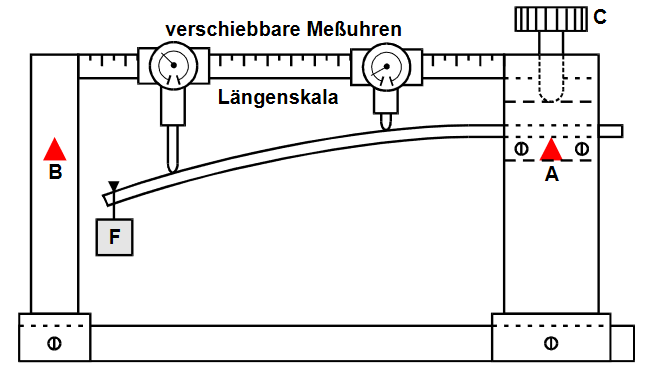
\includegraphics[width=0.7\textwidth]{assets/aufbau.png}
    \caption{Grundlegende Anordnung des Versuchsaufbaus \cite{V103}.}
    \label{fig:aufbau}
\end{figure}
Zur Bestimmung des Elastizitätsmodules wird der in \autoref{fig:aufbau} dargestellte Versuchsaufbau genutzt.
Ein Probestab wird dabei zunächst einseitig am Auflagepunkt A eingespannt während am freien Ende ein Gewicht angehängt wird.
Mit den verschiebbaren Messuhren kann nun an verschiedenen Stellen $x$ die Auslenkung $D$ abgelesen werden. Da die
Proben nicht perfekt gerade sind, wird dabei wie folgt vorgegangen:
Bevor das Gewicht angehängt wird, wird die Messuhr zunächst an die zu untersuchende Messstelle $x$ geschoben und auf $0$ geeicht.
Nun wird das Gewicht angehängt, sodass an der Messuhr direkt die Auslenkung abgelesen werden kann. Das Gewicht wird wieder entfernt
und die Messuhr wird zur nächsten Messstelle geschoben. Dieser Vorgang wird für insgesamt 20 verschiedene Messstellen durchgeführt.

\noindent In einer zweiten Messreihe wird der Probenstab beidseitig eingespannt. Das Gewicht wird in der Mitte des Stabes angehängt. In dieser
Messreihe werden beide Messuhren genutzt, sodass bei jedem Schritt jeweils ein Messwert links sowie rechts vom Gewicht abgelesen werden kann.
Wie zuvor werden die Messuhren zunächst ohne angehängtes Gewicht auf 0 geeicht. Dann wird das Gewicht angehängt und an den Messuhren wird die Auslenkung abgelesen.
Danach wird das Gewicht wieder abgenommen und die Messuhren werden zu den nächsten Messstellen geschoben. Insgesamt wird die Auslenkung an jeweils 10 verschiedenen
Messtellen auf beiden Seiten des Stabes bestimmt.

\noindent Am Ende wird der genutzte Stab gewogen und es wird sowohl die Länge als auch der Durchmesser (beim runden Probestab) bzw. die Kantenlängen (beim rechteckigen Stab)
der Stäbe notiert.

\noindent Die gesamte Messreihe wird für einen runden und einen rechteckigen Stab des selben Materials durchgeführt.